%矢量叉乘

\pentry{三阶行列式\upref{Deter}}

\subsection{叉乘的几何定义}

两个矢量 $\vec A$,  $\vec B$ 的\textbf{叉乘(cross product)}\footnote{也叫\textbf{叉积(cross product)},\textbf{向量积(vector product)}或\textbf{矢量积} },是一个矢量 $\vec C$.  叉乘用“ $\cross$” 表示,且\textbf{不可省略},即 $ \vec A \cross \vec B = \vec C$.要确定一个矢量,只需分别确定模长和方向.

\begin{enumerate}
\item $\vec C$ 的模长等于 $\vec A, \vec B$ 的模长之积与夹角 $\theta$ ($0\le\theta \le\pi$)的正弦值相乘.
\begin{equation}\label{Cross_eq1}
\abs {\vec C}  = \abs {\vec A} \abs {\vec B}  \sin \theta 
\end{equation}
\item $\vec C$ 的方向垂直于 $\vec A, \vec B$ 所在的平面,但一个平面有两个垂直方向,根据\textbf{右手定则} 决定是哪个.
\end{enumerate}
使用右手,并不是说“右”比“左”在数学上更加优越,而只是一种约定.这么约定跟我们的直角坐标系的定义方式有关.通常我们使用的直角坐标系如下面的右图所示,叫做右手系(左图中则是左手系).
\begin{figure}[h]
\centering
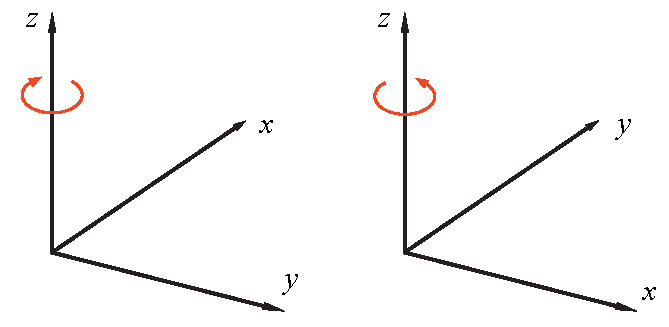
\includegraphics[width=10cm]{./figures/Cross.pdf}
\end{figure}
右(左)图之所以叫做右(左)手系,是因为把右(左)手的四指先指向 $x$ 轴,再弯向 $y$ 轴,竖起拇指,则拇指所指的方向就是 $z$ 轴.

按照上面的定义,在\textbf{右手系}中,三个坐标轴的单位矢量\footnote{模长为1的矢量} $\uvec x, \uvec y, \uvec z$ 满足
\begin{equation}\label{Cross_eq3}
\left\{ \begin{aligned}
\uvec x \cross \uvec y &= \uvec z\\
\uvec y \cross \uvec z &= \uvec x\\
\uvec z \cross \uvec x &= \uvec y
\end{aligned} \right.
\end{equation}
另外,跟点乘和数乘不同,叉乘\textbf{不满足交换律}.根据几何定义, $\vec B \cross \vec A$ 与 $\vec A \cross \vec B$ 模长相同,方向却相反.表示某个矢量的反方向,就是在前面加负号,所以有
\begin{equation}\label{Cross_eq11}
\vec B \cross \vec A = -\vec A \cross \vec B
\end{equation}
于是由关系\autoref{Cross_eq3} 可得
\begin{equation}\label{Cross_eq4}
\left\{ \begin{aligned}
\uvec y \cross \uvec x &=  - \uvec z\\
\uvec z \cross \uvec y &=  - \uvec x\\
\uvec x \cross \uvec z &=  - \uvec y
\end{aligned} \right.
\end{equation}
根据定义,一个矢量叉乘自身,模长为 $0$. 所以叉乘结果是零矢量 $\vec 0$. 于是又有
\begin{equation}\label{Cross_eq5}
\left\{ \begin{aligned}
\uvec x \cross \uvec x &= \vec 0\\
\uvec y \cross \uvec y &= \vec 0\\
\uvec z \cross \uvec z &= \vec 0
\end{aligned} \right.
\end{equation}
\autoref{Cross_eq3},\autoref{Cross_eq4} 和\autoref{Cross_eq5}中共9条式子,描述了 $\uvec x$,  $\uvec y$,  $\uvec z$ 任意两个叉乘的结果.

\subsection{叉乘与数乘的混合运算}

在 $\vec A \cross \vec B = \vec C$ 中, $\vec C$ 的方向仅由 $\vec A$ 和 $\vec B$ 的方向决定.当 $\vec A$ 和 $\vec B$ 的方向不变时, $\vec C$ 的模长正比 $\vec A$ 和 $\vec B$ 的模长相乘.假设 $\lambda $ 为常数(标量),显然有
\begin{equation}
(\lambda \vec A) \cross \vec B = \vec A \cross (\lambda \vec B) = \lambda (\vec A \cross \vec B)
\end{equation}
即标量的位置可以任意变换,但矢量与乘号的位置关系始终要保持不变.

\subsection{叉乘的分配律}

叉乘一个最重要的特性,就是它满足分配律.
\begin{equation}\label{Cross_eq6}
{\vec A} \cross (\vec B +\vec C) = {\vec A} \cross {\vec B} + {\vec A} \cross {\vec C}
\end{equation}
由\autoref{Cross_eq11} 及上式可以推出
\begin{equation}\label{Cross_eq7}
(\vec A + \vec B) \cross \vec C =  - \vec C \cross (\vec A + \vec B) =  - \vec C \cross \vec A - \vec C \cross \vec B = \vec A \cross \vec C + \vec B \cross \vec C
\end{equation}

在大部分的书上或课堂上,这个结论只是被简单地列出来,让学生觉得这是天经地义的(就因为这种运算叫做“\textbf{叉乘}”?).但从几何的角度理解,这个结论并不显然(见矢量叉乘分配律的几何证明\upref{CrossP})

\subsection{叉乘的坐标运算}

把矢量 $\vec A$ 和 $\vec B$ 分别在直角坐标系的三个单位矢量(也叫基底或矢基)展开,得到
\begin{equation}
\vec A = a_x\,\uvec x + a_y\,\uvec y + a_z\,\uvec z \qquad \vec B = b_x\,\uvec x + b_y\,\uvec y + b_z\,\uvec z
\end{equation}
$(a_x,a_y,a_z)$ 和 $(b_x,b_y,b_z)$ 分别是 $\vec A$ 和 $\vec B$ 的坐标.根据叉乘的分配律(\autoref{Cross_eq6} \autoref{Cross_eq7}),可得到如下9项
\begin{equation}
\begin{aligned}
\vec A \cross \vec B ={} &(a_x\,\uvec x + a_y\,\uvec y + a_z\,\uvec z) \cross (b_x\,\uvec x + b_y\,\uvec y + b_z\,\uvec z)\\
={} &+ {a_x}{b_x}(\uvec x \cross \uvec x) + {a_x}{b_y}(\uvec x \cross \uvec y) + {a_x}{b_z}(\uvec z \cross \uvec z)\\
&+ {a_y}{b_x}(\uvec y \cross \uvec x) + {a_y}{b_y}(\uvec y \cross \uvec y) + {a_y}{b_z}(\uvec y \cross \uvec z)\\
&+ {a_z}{b_x}\left( {\uvec z \cross \uvec x} \right) + {a_z}{b_y}\left( {\uvec z \cross \uvec y} \right) + {a_z}{b_z}\left( {\uvec z \cross \uvec z} \right)
\end{aligned}
\end{equation}
注意每一项中的运算在\autoref{Cross_eq3},\autoref{Cross_eq4} 和\autoref{Cross_eq5} 中都能找到答案,于是上式化为
\begin{equation}\label{Cross_eq2}
\vec A \cross \vec B = (a_y b_z - a_z b_y)\,\uvec x + (a_x b_z - a_z b_x)\,\uvec y + (a_x b_y - a_y b_x)\,\uvec z
\end{equation}
令 $\vec C = \vec A \cross \vec B$, 则 $\vec C$ 的分量表达式为
\begin{equation}
\left\{ \begin{aligned}
{c_x} &= {a_y}{b_z} - {a_z}{b_y}\\
{c_y} &= {a_x}{b_z} - {a_z}{b_x}\\
{c_z} &= {a_x}{b_y} - {a_y}{b_x}
\end{aligned} \right.
\end{equation}
\autoref{Cross_eq2} 可以用三阶行列式\upref{Deter}表示为
\begin{equation}
\vec A \cross \vec B = 
\begin{vmatrix}
{\uvec x} & {\uvec y} &{ \uvec z}\\
{a_x} & {a_y} & {a_z}\\
{b_x} & {b_y} & {b_z}
\end{vmatrix} \end{equation}
与普通行列式不同的是,这个行列式中的元有部分是矢量,所以得出的结果也是矢量.

\begin{exam}{}
空间直角坐标系中三角形的三点分别为 $O(0,0,0)$,  $A(1,1,0)$,  $B(-11,1)$. 求三角形的面积和一个单位法向量.

令 $O$ 到 $A$ 的矢量和  $O$ 到 $B$ 的矢量分别为
\begin{equation}\begin{aligned}
\vec a  &= (1,1,0) - (0,0,0) = (1,1,0)\\
\vec b  &= (-1,1,1) - (0,0,0) = (-1,1,1)
\end{aligned}\end{equation}
三角形的面积为
 \begin{equation}
{{S}} = \frac12 ab \sin \theta 
\end{equation}
其中 $\theta $ 是 $\vec a$ 与 $\vec b$ 的夹角.根据叉乘的几何定义中的\autoref{Cross_eq1}
\begin{equation}
{\rm{S}} = \frac 12 ab \sin \theta  = \frac 12 \abs{\vec a\cross\vec b}
\end{equation}
令
\begin{equation}
\vec v = \vec a \cross \vec b = 
\begin{vmatrix} {\uvec x}&{\uvec y}&{\uvec z}\\ 1&1&0\\-1&1&1 \end{vmatrix}
= \uvec x - \uvec y + 2\,\uvec z 
\end{equation}
坐标为 $(1,-1,2)$,模长为 $\abs{\vec v} = \sqrt {1 + 1 + {2^2}} = \sqrt 6$, 所以面积为 $S = \sqrt 6 /2$. 

根据叉乘的几何定义, $\vec v = (1,-1,2)$ 就是三角形的法向量,进行\textbf{归一化}\footnote{把矢量长度变为1,方向不变}
得单位法向量为
 \begin{equation}
\uvec v = \frac{\vec v}{\abs{\vec v}} = \frac{(1,-1,2)}{\sqrt 6 } = \left( \frac{\sqrt 6 }{6}, - \frac{\sqrt 6 }{6}, \frac{\sqrt 6 }{3} \,\right)
\end{equation}
\end{exam}
%例子: 绕轴旋转的线速度;洛伦兹力;安培力;%未完成:引用



